% Options for packages loaded elsewhere
\PassOptionsToPackage{unicode}{hyperref}
\PassOptionsToPackage{hyphens}{url}
%
\documentclass[
  12pt,
]{article}
\usepackage{lmodern}
\usepackage{amssymb,amsmath}
\usepackage{ifxetex,ifluatex}
\ifnum 0\ifxetex 1\fi\ifluatex 1\fi=0 % if pdftex
  \usepackage[T1]{fontenc}
  \usepackage[utf8]{inputenc}
  \usepackage{textcomp} % provide euro and other symbols
\else % if luatex or xetex
  \usepackage{unicode-math}
  \defaultfontfeatures{Scale=MatchLowercase}
  \defaultfontfeatures[\rmfamily]{Ligatures=TeX,Scale=1}
  \setmainfont[]{Times New Roman}
\fi
% Use upquote if available, for straight quotes in verbatim environments
\IfFileExists{upquote.sty}{\usepackage{upquote}}{}
\IfFileExists{microtype.sty}{% use microtype if available
  \usepackage[]{microtype}
  \UseMicrotypeSet[protrusion]{basicmath} % disable protrusion for tt fonts
}{}
\makeatletter
\@ifundefined{KOMAClassName}{% if non-KOMA class
  \IfFileExists{parskip.sty}{%
    \usepackage{parskip}
  }{% else
    \setlength{\parindent}{0pt}
    \setlength{\parskip}{6pt plus 2pt minus 1pt}}
}{% if KOMA class
  \KOMAoptions{parskip=half}}
\makeatother
\usepackage{xcolor}
\IfFileExists{xurl.sty}{\usepackage{xurl}}{} % add URL line breaks if available
\IfFileExists{bookmark.sty}{\usepackage{bookmark}}{\usepackage{hyperref}}
\hypersetup{
  pdftitle={Decadal trends in cadmium and lead concentrations in Mytilus edulis samples from several European nations},
  pdfauthor={Sena McCrory},
  hidelinks,
  pdfcreator={LaTeX via pandoc}}
\urlstyle{same} % disable monospaced font for URLs
\usepackage[margin=2.54cm]{geometry}
\usepackage{graphicx,grffile}
\makeatletter
\def\maxwidth{\ifdim\Gin@nat@width>\linewidth\linewidth\else\Gin@nat@width\fi}
\def\maxheight{\ifdim\Gin@nat@height>\textheight\textheight\else\Gin@nat@height\fi}
\makeatother
% Scale images if necessary, so that they will not overflow the page
% margins by default, and it is still possible to overwrite the defaults
% using explicit options in \includegraphics[width, height, ...]{}
\setkeys{Gin}{width=\maxwidth,height=\maxheight,keepaspectratio}
% Set default figure placement to htbp
\makeatletter
\def\fps@figure{htbp}
\makeatother
\setlength{\emergencystretch}{3em} % prevent overfull lines
\providecommand{\tightlist}{%
  \setlength{\itemsep}{0pt}\setlength{\parskip}{0pt}}
\setcounter{secnumdepth}{5}

\title{Decadal trends in cadmium and lead concentrations in \emph{Mytilus
edulis} samples from several European nations}
\usepackage{etoolbox}
\makeatletter
\providecommand{\subtitle}[1]{% add subtitle to \maketitle
  \apptocmd{\@title}{\par {\large #1 \par}}{}{}
}
\makeatother
\subtitle{\url{https://github.com/slm119/ENV872_FinalProject}}
\author{Sena McCrory}
\date{}

\begin{document}
\maketitle

\newpage
\tableofcontents 
\newpage
\listoftables 
\newpage
\listoffigures 
\newpage

\hypertarget{rationale-and-research-questions}{%
\section{Rationale and Research
Questions}\label{rationale-and-research-questions}}

\newpage

\hypertarget{dataset-information}{%
\section{Dataset Information}\label{dataset-information}}

\newpage

\hypertarget{exploratory-analysis}{%
\section{Exploratory Analysis}\label{exploratory-analysis}}

The ICES database includes \emph{Mytilus edulis} sample data from 1979
to 2018 for X European countries. Most samples were collected near
shorelines and within some enclosed bay or lake areas (Fig 1).

\begin{figure}
\centering
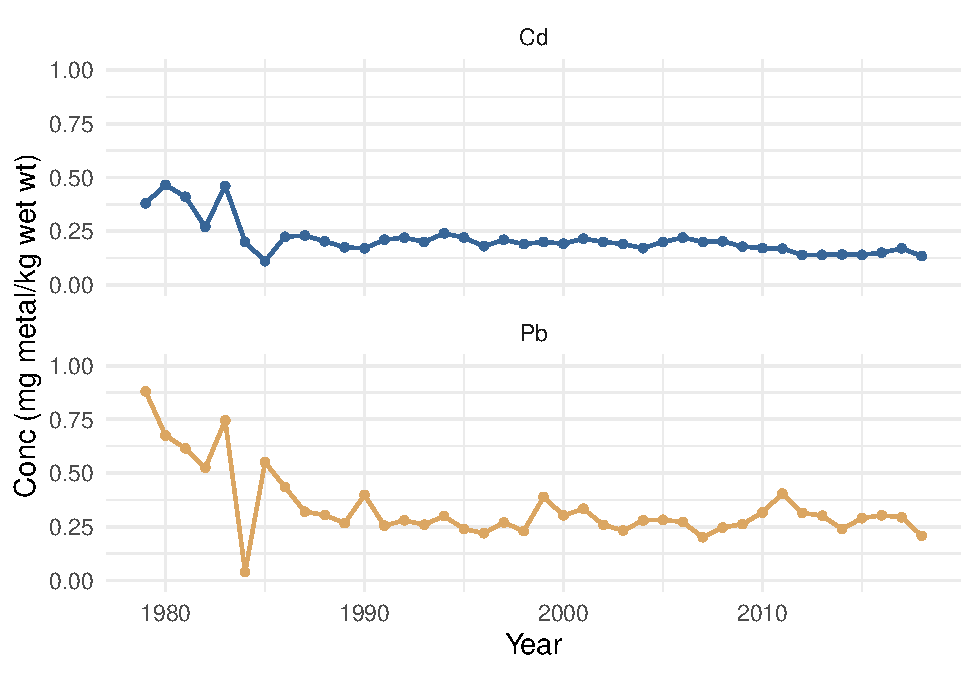
\includegraphics{McCrory_ENV972_Project_files/figure-latex/unnamed-chunk-1-1.pdf}
\caption{Yearly median concentrations of cadmium and lead in
\emph{Mytilus edulis} ICES monitoring data from 1979 to 2018.}
\end{figure}

\begin{figure}
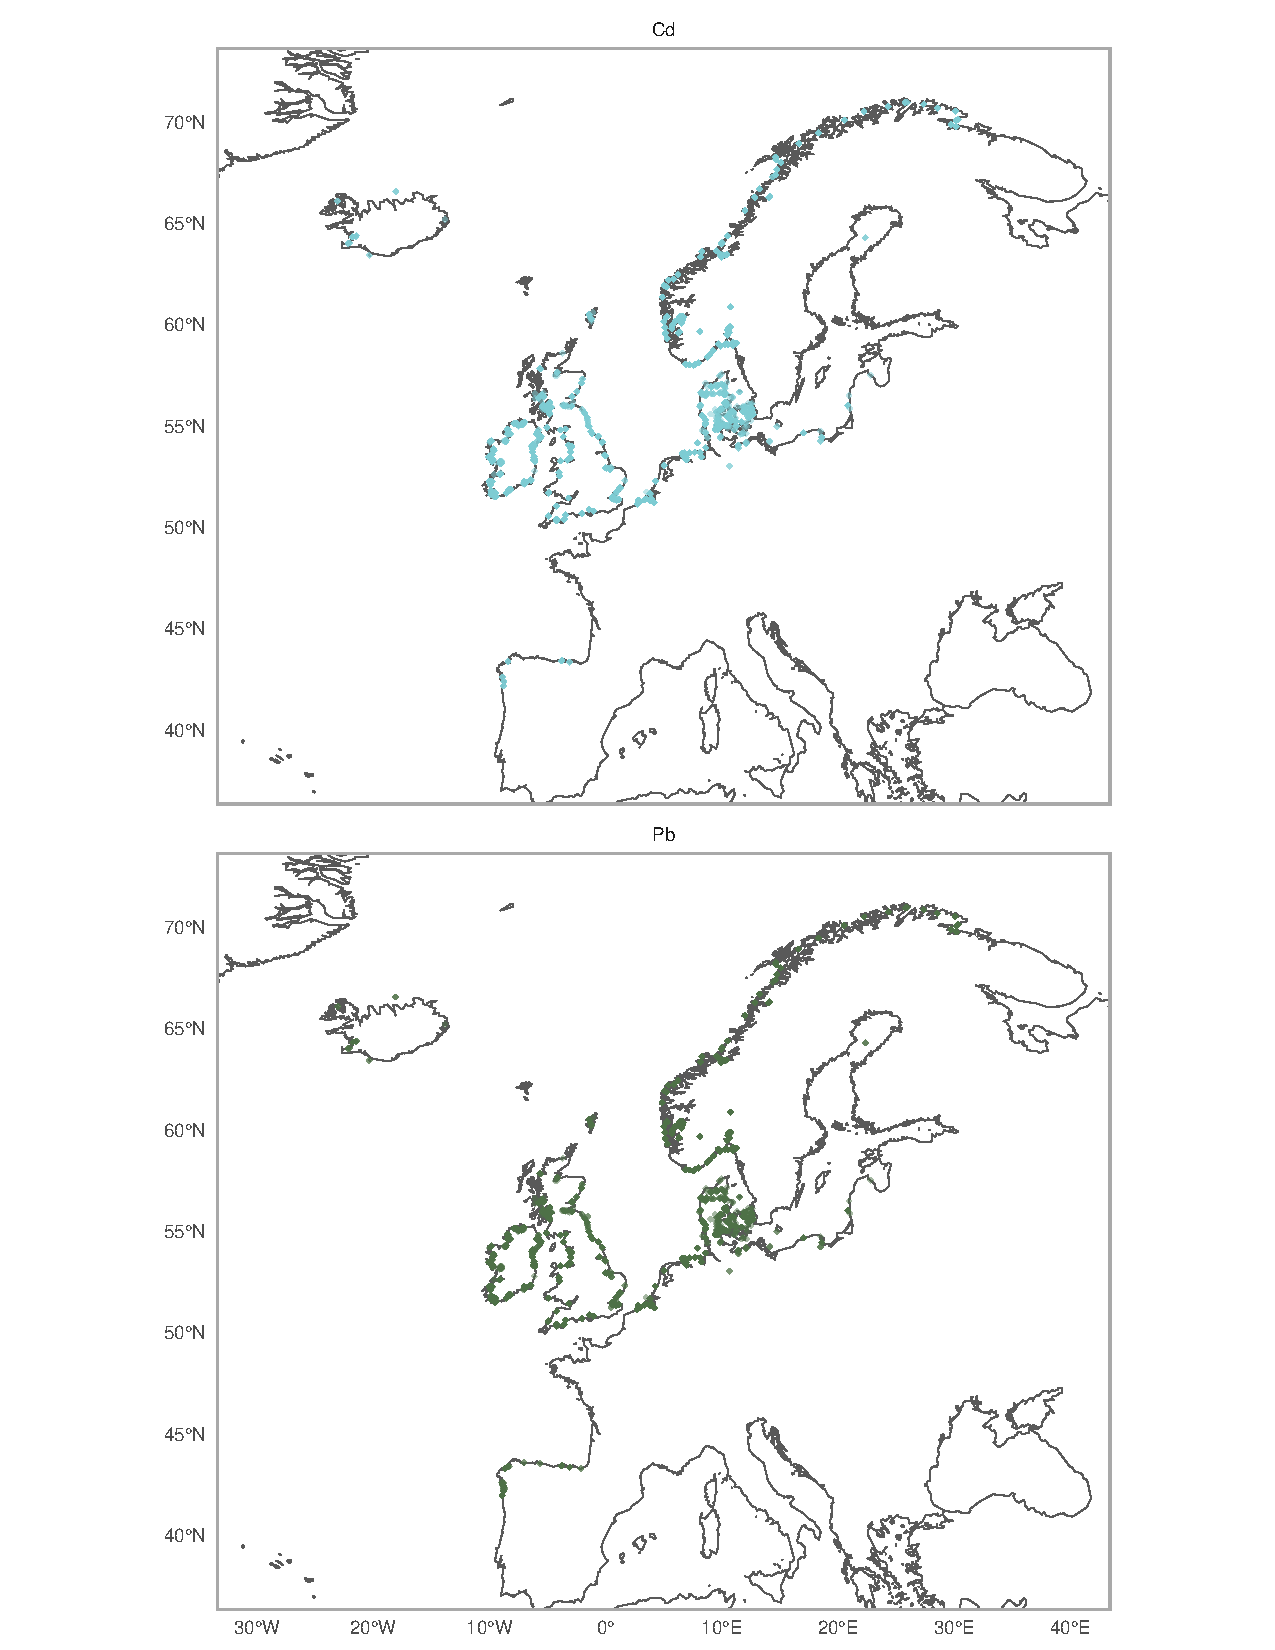
\includegraphics[width=0.9\linewidth]{C:/Users/senam/Box Sync/My Documents/MEM classes/Duke Spring 2020/DataAnalytics/ENV872_FinalProject/Output/StudyRegionMap} \caption{Sample locations from 1990 to 2018}\label{fig:unnamed-chunk-2}
\end{figure}

\begin{figure}
\centering
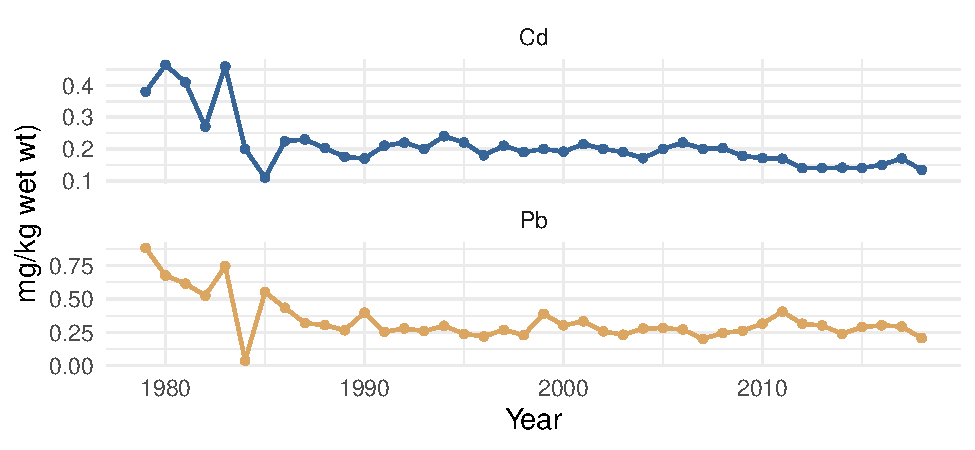
\includegraphics{McCrory_ENV972_Project_files/figure-latex/unnamed-chunk-3-1.pdf}
\caption{Distirbution of sample concentrations of cadmium and lead in
\emph{Mytilus edulis} from ICES data 1990 to 2019.}
\end{figure}

\begin{figure}
\centering
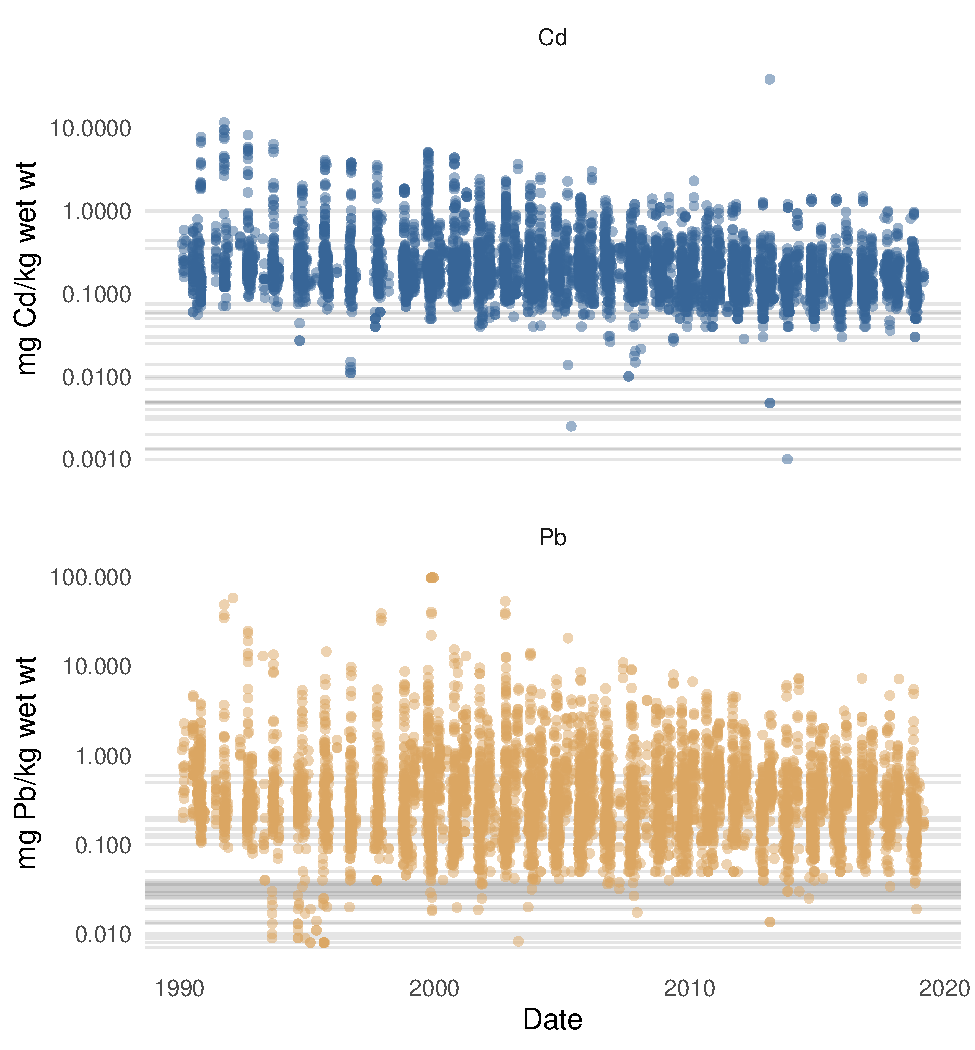
\includegraphics{McCrory_ENV972_Project_files/figure-latex/unnamed-chunk-4-1.pdf}
\caption{Cadmium and lead sample concentrations over time for ICES
\emph{Mytilus edulis} monitoring. Grey lines show the various instrument
detection limits reported in each the data set.}
\end{figure}

\newpage

\hypertarget{analysis}{%
\section{Analysis}\label{analysis}}

\hypertarget{question-1-how-have-cadmium-and-lead-concentrations-in-mytilus-edulis-changed-over-time}{%
\subsection{\texorpdfstring{Question 1: How have cadmium and lead
concentrations in \emph{Mytilus edulis} changed over
time?}{Question 1: How have cadmium and lead concentrations in Mytilus edulis changed over time?}}\label{question-1-how-have-cadmium-and-lead-concentrations-in-mytilus-edulis-changed-over-time}}

\begin{figure}
\centering
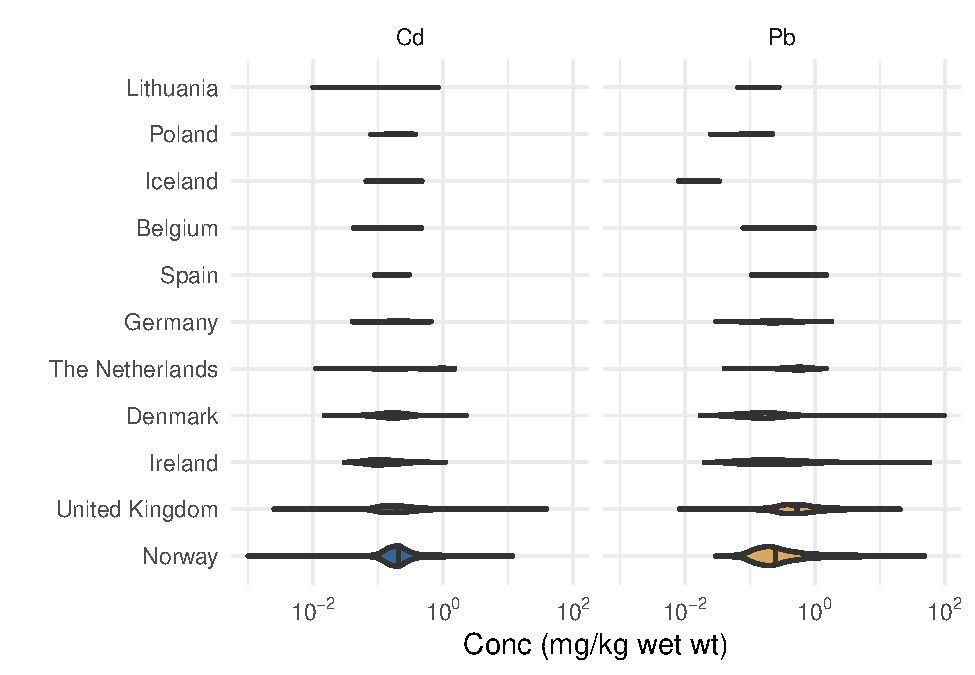
\includegraphics{McCrory_ENV972_Project_files/figure-latex/unnamed-chunk-5-1.pdf}
\caption{Concentrations of cadmium and lead in \emph{Mytilus edulis} in
ICES study region from 1990 to 2018.}
\end{figure}

\hypertarget{question-2-do-cadmium-and-lead-concentrations-in-mytilus-edulis-differ-by-country}{%
\subsection{\texorpdfstring{Question 2: Do cadmium and lead
concentrations in \emph{Mytilus edulis} differ by
country?}{Question 2: Do cadmium and lead concentrations in Mytilus edulis differ by country?}}\label{question-2-do-cadmium-and-lead-concentrations-in-mytilus-edulis-differ-by-country}}

\begin{figure}
\centering
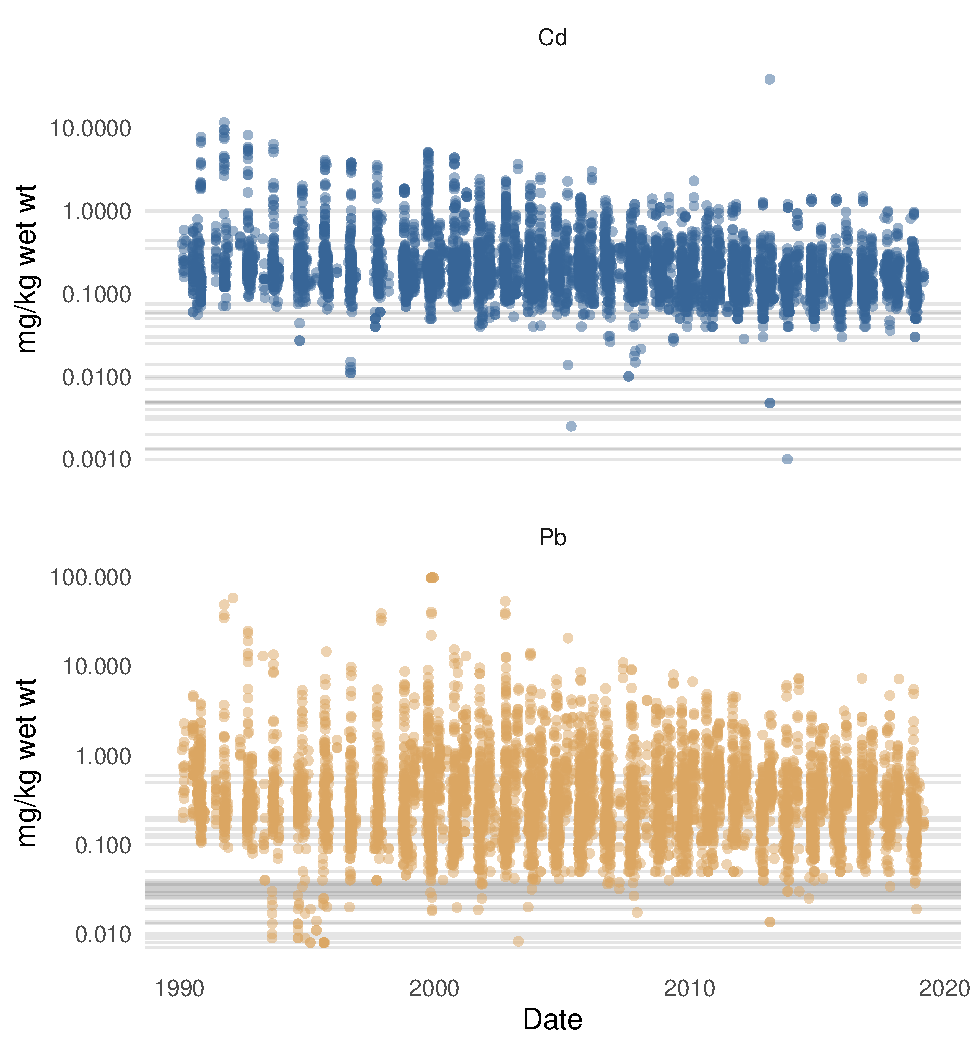
\includegraphics{McCrory_ENV972_Project_files/figure-latex/unnamed-chunk-6-1.pdf}
\caption{Concentrations of cadmium and lead in \emph{Mytilus edulis} for
countries with more than 100 samples between 1990 and 2018.}
\end{figure}

\newpage

\hypertarget{summary-and-conclusions}{%
\section{Summary and Conclusions}\label{summary-and-conclusions}}

\newpage

\hypertarget{references}{%
\section{References}\label{references}}

\textless add references here if relevant, otherwise delete this
section\textgreater{}

\end{document}
